\chapter{Taylor and Maclaurin Series}

Consider the generic power series:
$$f(x) = c_0 + c_1(x - a) + c_2(x - a)^2 + c_3(x - a)^3 + \cdots + c_n(x - a)^n$$
Notice that substituting $x = a$ yields:
$$f(a) = c_0$$
Suppose we differentiate both sides, which gives:
$$f'(x) = c_1 + 2c_2(x - a) + 3c_3(x - a)^2 + \cdots nc_n(x-a)^{n-1}$$
Again, substituting $x = a$:
$$f'(a) = c_1$$
Continuing, we see that
$$f''(x) = 2c_2 + 2 \cdot 3c_3(x-a) + \cdot + sn(n-1)(x-a)^{n-2}$$
And
$$f''(a) = 2c_2$$
Once more, we see that:
$$f'''(x) = 2 \cdot 3 c_3 + 2 \cdot 3 c\dot 4 (x-a) + \cdots + n (n-1)(n-2)(x-a)^{n-3}$$
And substituting $x = a$ gives
$$f'''(a) = 2 \cdot 3 c_3 = 3!c_3$$

Do you see the pattern? It is 
$$f^{(n)}(a) = 2 \cdot 3 \cdot 4 \cdot \cdots \cdot nc_n = n!c_n$$
Which also means that 
$$c_n = \frac{f^{(n)}(a)}{n!}$$
(recall the convention that $0! = 1$, so this is valid for $n = 0$ as well). 

If we substitute for $c_n$ into our definition of a power series, we get a \textbf{Taylor series}\index{Taylor series}:
$$f(x) = \sum_{n=0}^\infty \frac{f^{(n)}(a)}{n!} \left( x - a \right)^n$$

This is called the \textit{Taylor series of $f$ centered at $a$}. If $a = 0$, we call this special case a \textbf{Maclaurin series}\index{Maclaurin series}:
$$f(x) = \sum_{n=0}^\infty \frac{f^{(n)}(0)}{n!}x^n$$

\textbf{Example}: Find the Maclaurin series for $f(x) = e^x$ and its radius of convergence.

\textbf{Solution}: We know that if $f(x) = e^x$, then $f'(x) = e^x$, and $f''(x) = e^x$, $\cdots$, $f^{(n)}(x) = e^x$. Since $e^0 = 1$, we can say that $f^{(n)}(0) = 1$ for all $n$. Substituting this into our equation for Maclaurin series:
$$f(x) = \sum_{n=0}^\infty \frac{f^{(n)}(0)}{n!}x^n = \sum_{n=0}^\infty \frac{1}{n!}x^n $$
$$= \sum_{n=0}^\infty \frac{x^n}{n!}$$

Taking $a_n = \frac{x^n}{n!}$ and applying the Ratio test, we can find the radius of convergence:
$$\lim_{n \to \infty} \left| \frac{a_{n + 1}}{a_n} \right| < 1$$
$$\lim_{n \to \infty} \left| \frac{x^{n + 1}}{(n+1)n!} \cdot \frac{n!}{x^n} \right| < 1$$
$$\lim_{n \to \infty} \frac{|x|}{n + 1} = 0 < 1$$
The limit converges to 0 for all $x$, so the radius of convergence is $\infty$. 

We can confirm this graphically. But first, a quick definition. The $n^{th}$-degree Taylor polynomial is the first $n$ terms of the infinite Taylor polynomial. That is,
$$T_n(x) = \sum_{i=0}^n \frac{f^{(n)}(a)}{i!}(x - a)^n$$

In the case of $f(x) = e^x$ and $a = 0$, the $n^{th}$ degree Taylor polynomial is given by:
$$T_n(x) = \sum_{i = 0}^\infty \frac{x^i}{i!}$$
As expected, as the degree of the polynomial increases, the closer it is to $e^x$ (see figure \ref{taylorexp}).

\begin{figure}[htbp]
\centering
    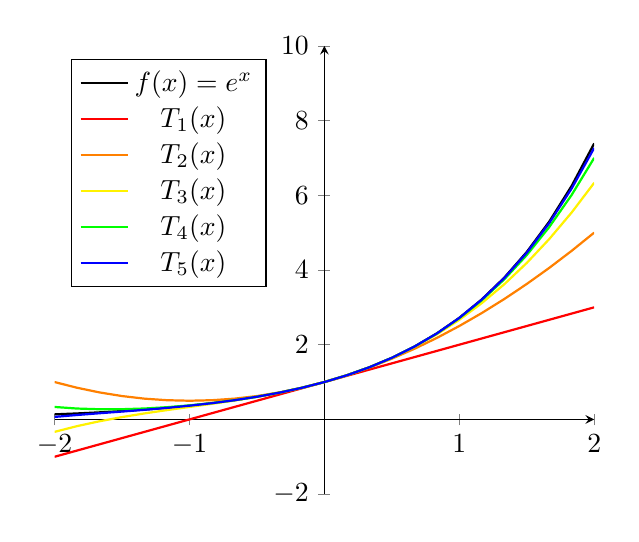
\begin{tikzpicture}
	\begin{axis}[xmin = -2, xmax = 2, axis lines = center, ymin = -2, ymax = 10, legend pos = north west]
        \addplot[black, thick, domain = -2:2]{e^x};
        \addlegendentry{$f(x) = e^x$};
        \addplot[red, thick, domain = -2:2]{1 + x};
        \addlegendentry{$T_1(x)$};
        \addplot[orange, thick, domain = -2:2]{1 + x + x^2/2};
        \addlegendentry{$T_2(x)$};
        \addplot[yellow, thick, domain = -2:2]{1 + x + x^2/2 + x^3/6};
        \addlegendentry{$T_3(x)$};
        \addplot[green, thick, domain = -2:2]{1 + x + x^2/2 + x^3/6 + x^4/24};
        \addlegendentry{$T_4(x)$};
        \addplot[blue, thick, domain = -2:2]{1 + x + x^2/2 + x^3/6 + x^4/24 + x^5/120};
        \addlegendentry{$T_5(x)$};
        \end{axis}
    \end{tikzpicture}
    \caption{As $n$ increases, $T_n(x)$ approaches $f(x)$}
    \label{taylorexp}
\end{figure}

\section{Maclaurin series of trigonometric functions}
Let us write a Maclaurin series for $\sin{x}$. 

\begin{Exercise}[label = mac1]
[The problem was originally presented as a no-calculator, multiple-choice 
question on the 2012 AP Calculus BC exam.] The Maclaurin series for the 
function $f$ is given by $f(x) = \sum_{n=0}^\infty \left( -\frac{x}{4} \right)^
n$. What is the value of $f(3)$?
\end{Exercise}

\begin{Answer}[ref = mac1]
Substituting $x = 3$, the series is $\sum_{n=0}^\infty \left( -\frac{3}{4} 
\right)^n$, which is an alternating geometric series. Reindexing the series to 
begin at $n = 1$, this is equivalent to $\sum_{n = 1}^\infty \left( - 
\frac{3}{4} \right) ^ {n - 1}$, which is in the standard form $\sum_{n=1}^
\infty ar^{n-1}$ with $a = 1$ and $r = -\frac{3}{4}$. Then the value of the 
series is $\frac{a}{1-r} = \frac{1}{1-\left(- \frac{3}{4} \right)} = \frac{1}{1 
+ \frac{3}{4}} = \frac{1}{\frac{7}{4}} = \frac{4}{7}$. 
\end{Answer}

\begin{Exercise}[label = taylor1]
[This problem was originally presented as a calculator-allowed, multiple-choice 
question on the 2012 AP Calculus BC exam.] Let $f$ be function having 
derivatives of all orders for $x > 0$ such taht $f(3) = 2$, $f'(3) = -1$, 
$f''(3) = 6$, and $f'''(3) = 12$. Write a $3^{rd}$-degree Taylor polynomial 
for $f$ about $x = 3$ and estimate the value of $f(3.4)$
\end{Exercise}

\begin{Answer}[ref = taylor1]
A third-degree Taylor polynomial about $x = 3$ is given by $f(3) + \frac{
f'(3)}{1!} (x - 3) + \frac{f''(3)}{2!} (x - 3) ^ 2 + \frac{f'''(3)}{3!} (x - 3) 
^ 3$. Substituting what we know, they 3rd-degree Taylor polynomial is $f(x) 
\approx 2 + \frac{-1}{1} (x - 3) + \frac{6}{2} (x - 3) ^ 2 + \frac{12}{6}(x - 
3) ^ 3 = 2 - (x - 3) + 3 (x - 3) ^ 2 + 2 (x - 3) ^ 3$. Substituting $x = 3.5$, 
we find that $f(3.5) \approx 2 - (3.5 - 3) + 3 ( 3.5 - 3) ^ 2 + 2 (3.5 - 3) ^ 3 
= 2 - \frac{1}{2} + 3 \frac{1}{4} + 2\frac{1}{8} = 2 - \frac{1}{2} + 
\frac{3}{4} + \frac{1}{4} = 2.5$.
\end{Answer}

\begin{Exercise}[label = taylor2]
[This problem was originally presented as a calculator-allowed, free-response 
question on the 2012 AP Calculus BC exam.] The function $f$ is twice 
differentiable for $x > 0$ with $f(1) = 15$, $f'(1) = 8$, and $f''(1) = 20$. 
Write the second-degree Taylor polynomial about $x = 1$ and use it to 
estimate $f(1.4)$.
\end{Exercise}

\begin{Answer}
A second-degree Taylor polynomial about $x = 1$ is given by $f(x) \approx f(1) 
+ \frac{f'(1)}{1!}(x - 1) + \frac{f''(1)}{2!}(x - 1)^2 = 15 + 8(x - 1) + 10(x 
- 1)^2$. Substituting $x = 1.4$, we find that $f(1.4) \approx 15 + 8(1.4 - 1) 
+ 10(1.4 - 1)^2 = 19.8$.
\end{Answer}


